% ch21: 导数的应用
\chapter{导数的应用——极值、凹凸、作图}
\begin{applicationbox}
学完本章：用导数分析函数——找极值、判断凹凸、完整作图
\end{applicationbox}

\section{极值}
\(f'(x)=0\) 的点叫\textbf{驻点}。若 \(f'\) 由正变负则为极大值，由负变正则为极小值。

\textbf{费马定理的 ε-δ 证明：} 设 \(f\) 在 \(x=c\) 处取局部极大值，则存在 \(\delta>0\) 使 \(|x-c|<\delta\) 时 \(f(x)\le f(c)\)。
对 \(h\in(0,\delta)\)，\(\frac{f(c+h)-f(c)}{h}\le0\)，取极限得 \(f'(c)\le0\)。
对 \(h\in(-\delta,0)\)，\(\frac{f(c+h)-f(c)}{h}\ge0\)，取极限得 \(f'(c)\ge0\)。
故 \(f'(c)=0\)。\(\blacksquare\)

\textbf{单调性的 ε-δ 判别：} 若 \(f'(x)>0\) 恒成立，则由拉格朗日中值定理，
对任意 \(x_1<x_2\)，存在 \(c\in(x_1,x_2)\) 使 \(f(x_2)-f(x_1)=f'(c)(x_2-x_1)>0\)，故 \(f\) 严格递增。\(\blacksquare\)

\begin{center}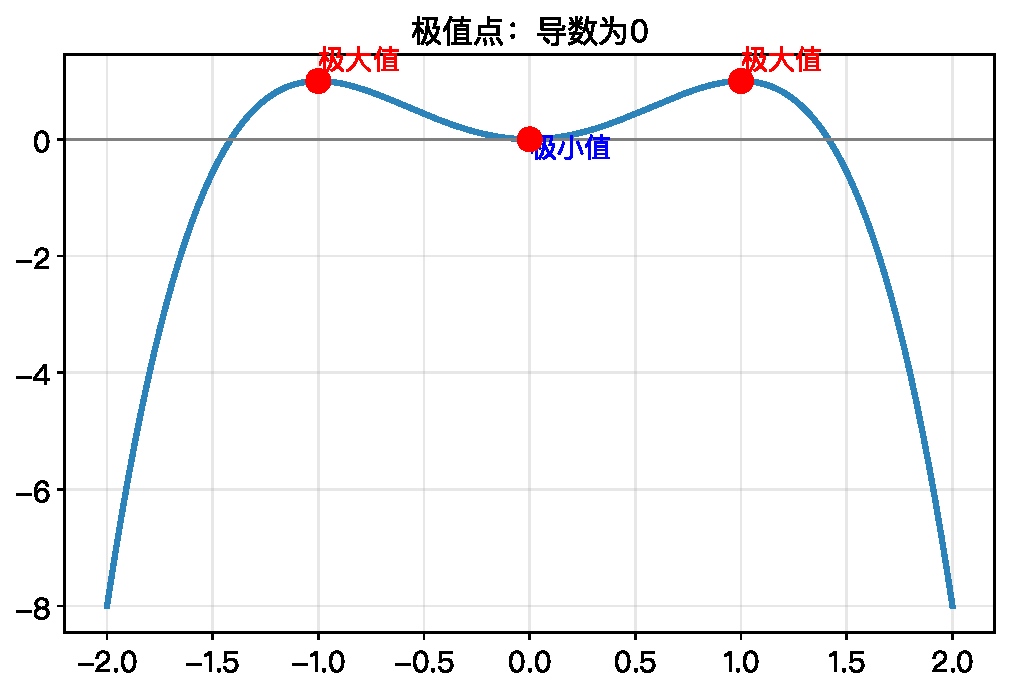
\includegraphics[width=0.6\textwidth]{figures/ch21_extrema.pdf}\end{center}

\section{凹凸性与拐点}
\(f''(x)>0\) 为凹（开口向上），\(f''(x)<0\) 为凸（开口向下）。\(f''(x)=0\) 且变号处为\textbf{拐点}。

\begin{center}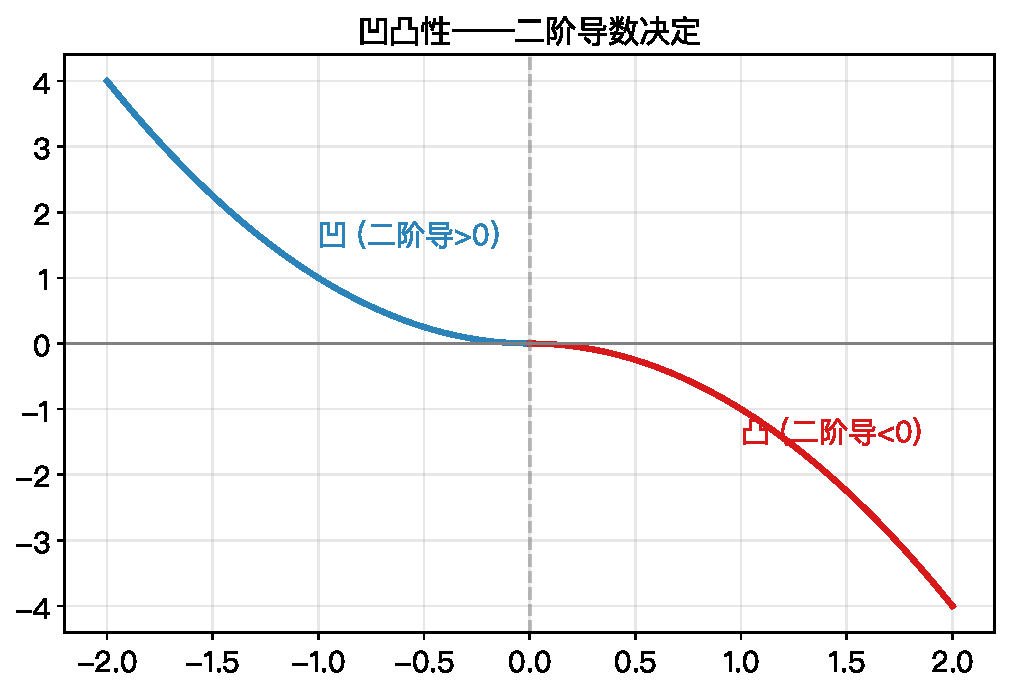
\includegraphics[width=0.6\textwidth]{figures/ch21_concavity.pdf}\end{center}

\section{函数作图的完整流程}
\begin{enumerate}
\item 确定定义域、对称性
\item 求 \(f'(x)\) 找驻点和单调区间
\item 求 \(f''(x)\) 找拐点和凹凸区间
\item 求渐近线
\item 列表、描点、连线
\end{enumerate}

\section{习题}
\begin{exercise}[0] \(f'(x)=0\) 的点叫什么？\end{exercise}
\begin{exercise}[0] \(f''(x)>0\) 表示函数是凹还是凸？\end{exercise}
\begin{exercise}[0] 极大值点的导数一定为0吗？\end{exercise}
\begin{exercise}[0] 拐点处 \(f''(x)\) 等于多少？\end{exercise}
\begin{exercise}[1] 求 \(f(x)=x^2-4x+3\) 的极值。\end{exercise}
\begin{exercise}[1] 判断 \(f(x)=x^3\) 在 \(x=0\) 处是否有极值。\end{exercise}
\begin{exercise}[1] 求 \(f(x)=x^3-3x\) 的极值点。\end{exercise}
\begin{exercise}[1] 求 \(f(x)=x^2\) 的凹凸性。\end{exercise}
\begin{exercise}[2] 求 \(f(x)=2x^3-3x^2-12x+1\) 的极值。\end{exercise}
\begin{exercise}[2] 求 \(f(x)=x^3-6x^2\) 的凹凸区间和拐点。\end{exercise}
\begin{exercise}[2] 求 \(f(x)=x+\frac{1}{x}\) 的极值。\end{exercise}
\begin{exercise}[2] 求证 \(e^x \ge x+1\)。\end{exercise}
\begin{exercise}[3] 求 \(f(x)=x^4-4x^3\) 的极值和拐点。\end{exercise}
\begin{exercise}[3] 求 \(f(x)=x\ln x\) 的极值。\end{exercise}
\begin{exercise}[3] 求 \(f(x)=\frac{x^2}{1+x^2}\) 的渐近线。\end{exercise}
\begin{exercise}[3] 求内接于圆的最大矩形面积。\end{exercise}
\begin{exercise}[3] 做一个容积为 \(V\) 的无盖圆柱形水桶，求最小表面积。\end{exercise}
\begin{exercise}[4] 求 \(f(x)=x^2e^{-x}\) 的极值和拐点。\end{exercise}
\begin{exercise}[4] 求 \(f(x)=\ln(1+x^2)\) 的凹凸区间。\end{exercise}
\begin{exercise}[4] 求 \(f(x)=\frac{x}{x^2-1}\) 的渐近线。\end{exercise}
\begin{exercise}[4] 围栏长100米，靠墙围最大矩形面积。\end{exercise}
\begin{exercise}[4] 证明 \(x^3-3x+1=0\) 在 \((0,1)\) 内恰有一个根。\end{exercise}
\begin{exercise}[5] 求 \(f(x)=e^{-x^2}\) 的极值、凹凸、拐点。\end{exercise}
\begin{exercise}[5] 作 \(f(x)=\frac{x}{1-x^2}\) 的完整图像。\end{exercise}
\begin{exercise}[5] 求 \(f(x)=x-\arctan x\) 的凹凸区间。\end{exercise}
\begin{exercise}[5] 证明 \(\ln(1+x) \le x\)（\(x>-1\)）。\end{exercise}
\begin{exercise}[6] 作 \(f(x)=x^{1/x}\)（\(x>0\)）的图像。\end{exercise}
\begin{exercise}[6] 求 \(f(x)=\frac{e^x}{x}\) 的完整图像分析。\end{exercise}
\begin{exercise}[6] 证明 \(x^\alpha \le \alpha x + (1-\alpha)\)（\(x>0, 0<\alpha<1\)）。\end{exercise}
\begin{exercise}[7] 求 \(f(x)=\frac{x^3}{(x-1)^2}\) 的完整图像分析（含渐近线）。\end{exercise}
